%!TEX root = ../template.tex
%%%%%%%%%%%%%%%%%%%%%%%%%%%%%%%%%%%%%%%%%%%%%%%%%%%%%%%%%%%%%%%%%%%%
%% chapter2.tex
%% NOVA thesis document file
%%
%% Chapter with the template manual
%%%%%%%%%%%%%%%%%%%%%%%%%%%%%%%%%%%%%%%%%%%%%%%%%%%%%%%%%%%%%%%%%%%%
\chapter{Related Work}
\label{cha:related_work}

This chapter presents and briefly discusses the related work and the study performed beforehand in order to guide and give some context to the reader. It will present work that was used as the basis of this thesis, existent technologies and their relation with this project, and some comparisons between those existing technologies, the problem addressed in this thesis and the solutions proposed to solve, or better address, those very same problems.

First, in section \ref{sec:key-value_stores} we explain and discuss for the first time the definition of a Key-Value Store. We present some use cases, current technology available, their differences and most importantly their security models and concerns.
Having discussed the software, section \ref{sec:trusted_computing _environments} will then address the environment on where that software will run on, most specifically the hardware. It explains and present the different ways to secure and authenticate the hardware, prevent hardware-based attacks and discuss some of the current products available and how they will be used across this thesis.
Section \ref{sec:sgx_enabled_key_value_stores} will then make the bridge between software and hardware. It explains how Key-Value stores are currently being run on secure environments. It discusses how software and hardware work together to achieve a secure application.
This chapter will be focused on the Intel SGX secure model and explain the advantages and disadvantages of this module.
To conclude the chapter, section \ref{sec:related_work_balance_and_critical_analysis} will combine the information of every sub-chapter and analyze it with a bigger perspective and better knowledge of the theme.

Section \ref{sec:sgx_enabled_key_value_stores} is considered to be the \textbf{main core} investigation and directly related to the work planned for this thesis. As for the other sections, they provide a background knowledge necessary for understanding of the core of this dissertation.

Along the next chapter we summarise the main relevant ideas that can be retained from each section for our objectives and expected goals.

\section{Key-Value Stores} % (fold)
\label{sec:key-value_stores}

Key value stores are the simplest form of what computer scientists call a database. The simplicity lies on associating a value to a certain key and storing that pair, as well as retrieving the values of known keys. \cite{db-engine:1}

\lstset{language=Bash, caption=Redis Set \& Get, label=lst:redisSetGet}
\begin{lstlisting}
redis> SET mykey "Hello"
"OK"
redis> GET mykey
"Hello"
\end{lstlisting}

Is this simplicity that makes this technology very attractive to developers. The ease of use, its high performance and speed are key aspects in favour of this technologies. However, simply working with keys and values might not be enough to more complex applications, and that is why Key-Value store product developers are introducing new features in order to make them appealing to a broader mass of users, always keeping them lightweight and fast.

For that lightweight and fast attributes, most of the key-value stores work in the computer memory. This allows fast get and write operations as opposed to persistent disk storage. Although they work mainly in memory, most of the solutions offer some persistent mechanism so we can make use of its performance but still persist data in case of a disaster, server failure or any crash.

\glspl{KVS} have been evolving for years and some are now more than a single key-value store module. A lot of them are now supporting a multi-model storage. Meaning that a value can be more than a single integer or a string. For example, Redis \cite{redis:1} as a multi-model store is not only a key-value store, but also \cite{redis:2}:

\begin{itemize}
	\item \textbf{Document Store} - \textit{"nonrelational database that is designed to store and query data as JSON-like documents"} \cite{aws-nosql:1}
	\item \textbf{Graph \gls{DBMS}} - \textit{"Graph databases are purpose-built to store and navigate relationships. Use nodes to store data entities, and edges to store relationships between entities"} \cite{aws-nosql:2} 
	\item \textbf{Search Engine} - \textit{"nonrelational database that is dedicated to the search of data content. Use indexes to categorize the similar characteristics among data"} \cite{aws-nosql:3} 
	\item \textbf{Time Series \gls{DBMS}} - \textit{"Provides optimum support for working with time-dependent data. Each entry has a timestamp, the data arrives in time order and time represents a primary axis for the information."} \cite{timeSeries:1}
\end{itemize}

So, the \gls{KVS} world is becoming more and more versatile as the years pass.

In the next subsections its discussed and presented the overview of the current \gls{KVS} technology. We picked the some top KVSs technologies nowadays according to db-engines \cite{db-engine:2} website.

\subsection{Memcached} % (fold)
\label{ssec:memcached}

Memcached \cite{memcached:1} is a free and open source key-value store released in 2003. It is described as a high performance distributed memory object caching system.

It is design to hold small chunks of data (strings and objects) to work as a cache for results of database calls, API calls, or page rendering. Its biggest use case is for use in speeding up dynamic web applications by alleviating database load.

This system lies on the simpler key-value store spectrum. It takes advantages of the simplicity of a key-value store to edge ease of development, and solving many problems facing large data caches. Its API is available for most popular languages. It has a \gls{LRU} eviction technique which means that items will expire after a specified amount of time if not used. 

When it comes to system replication, availability and reliability, Memcached has an interesting approach. In order to keep it blazing fast, there is no communication between server instances in a cluster. Memcached servers are unaware of each other. There is no crosstalk, no synchronization, no broadcasting, no replication. Adding servers will only increase the available memory.

As for its security context, Memcached spends very little, if any, effort in securing the systems for random internet connections. The servers only have support for SASL \cite{sasl:1} authentication mechanism. This method of authentication is not implemented as end-to-end encryption, it only provides restriction access to the daemon, but it does not hide communications over the network. That means it is not meant to be exposed to the internet or to any untrusted users \cite{memcached:2}.

\subsection{Redis} % (fold)
\label{ssec:redis}

Redis \cite{redis:1} is an in-memory data structure store that can be used as a database, cache and also a message broker. Redis focuses on performance, so most of its decisions prioritize high performance and very low latency.

It has been benchmarked as the world's fastest database \cite{redis:3} and together with a their multi-model and its rich set of operations that can be performed over data it has been the leading key-value store according to use and popularity for a multiple set of years \cite{db-engine:2}.

\lstset{language=Bash, caption=How Fast is Redis, label=lst:redisBenchmark}
\begin{lstlisting}
$ redis-benchmark -t set -r 100000 -n 1000000
====== SET ======
1000000 requests completed in 8.78 seconds
50 parallel clients
3 bytes payload
keep alive: 1

99.59% <= 1 milliseconds
99.98% <= 2 milliseconds
100.00% <= 2 milliseconds
113934.14 requests per second
\end{lstlisting}

As said before, Redis is now not a simple \gls{KVS}. It supports data structures such as strings, hashes, lists, sets, sorted sets with range queries, bitmaps, hyperloglogs, geospatial indexes with radius queries and streams. It also has built-in replication, server side scripting, \gls{LRU} eviction, concept of transactions and different levels of persistence. It provides high availability and automatic partitioning as well.

Redis provides replication in form of a master-slave model. This form of replication works with a single node (master node) where all writes occurring will be replicated to the other Redis instances (slave nodes). Writes on nodes other than the master will not be replicated. Redis provides a read-only setting that can be applied to slave nodes to prevent states differences between instances.

Security is not Redis' primarily concern (just like others). \textit{"In general, Redis is not optimised for maximum security but for maximum performance and simplicity"} \cite{redis:4}. It is design to be access by trusted clients inside trusted networks. This means that it is not supposed to be publicly exposed. Redis implements a simple authentication system with a password on the configuration file for client authentication.
It is also advised to run it behind a proxy to enable some \gls{ACL} policies and \gls{SSL} network security.

There are a few other security concerns that Redis addresses, but has we can now start to see, in this types of stores, security falls behind performance and usability.

\subsection{Amazon Dynamo DB}
\label{ssec:amazon_dynamo_db}

Amazon Dynamo DB \cite{dynamo:1} is a fully managed NoSQL database service. It is a key-value store and a document store that is built based on the dynamo paper \cite{dynamo:2}. This paper describes a \gls{P2P} (peer-to-peer) network with high availability, eventual consistency and very easily scalable. It also successful handles server and data center failures and network partitions.

Amazon builds on this paper and offers DynamoDB as a service in their platform. It is a hosted system in the Amazon Web Services \cite{aws:1} infrastructure and it is fully managed. That means no need for low level server configurations or maintenance. It is all managed by the \gls{AWS} team and offered to the user with a nice configuration interface. It also means that it has built-in security, backup and restore and in-memory caching for internet-scale applications. It also offers seamless scalability by increasing the number of nodes/servers according to current traffic received by the application on any given time. 

This technology focuses more on high availability but also achieves very high performances and very low latency and being fully managed it also takes advantages of the \gls{AWS} infrastructure full power. It currently sits second on the db-engines \cite{db-engine:2} most popular ranking.

\subsection{Microsoft Azure Cosmos DB}
\label{ssec:microsoft_azure_cosmos_db}

Microsoft Azure Cosmos DB \cite{cosmos:1} is a fully managed database service provided by Microsoft Azure \cite{azure:1}. This service provides a global distributed, horizontally scalable, multi-model database. Its multi-model architecture can work as a key-value store, a Document Store, a graph \gls{DBMS} and a wide column store.

It's very proud and excels in the easy of global scale with the system call \textit{Turnkey global distribution}, providing transparent multi-master replication and a set of users configurable consistency options. It also strongly advertises a \textit{Multi-Model Multi-Api} feature where you can use multiple data types on this single database service. Cosmos DB automatically indexes all data and allows the user to use various NoSQL APIs to query the data.

As a fully managed service, Cosmos DB makes use, in the background, of the large infrastructure with almost unlimited resources and capabilities provided by Microsoft, which means it also has built-in security, fail-over mechanisms for disaster recovery, and high performance with single digit read and write latencies.

\subsection{Microsoft Azure Cache for Redis}
\label{ssec:microsoft_azure_cache_for_redis}

Microsoft Azure Cache for Redis \cite{cache-for-redis:1} is a service provided by Microsoft Azure that joins the open source world of Redis with the commercial side of a fully managed and hosted platform.

It uses at its core the Redis server technology and provides ease of deployment and management, built-in global replication, Azures' infrastructure security and flexible scaling and Redis superior throughput and low latency performance.

Being in the Azure ecosystem provides nice integration with all Azures' services as shown in figure \ref{fig:azure_ecosystem}.

\begin{figure}[htbp]
	\centering
	{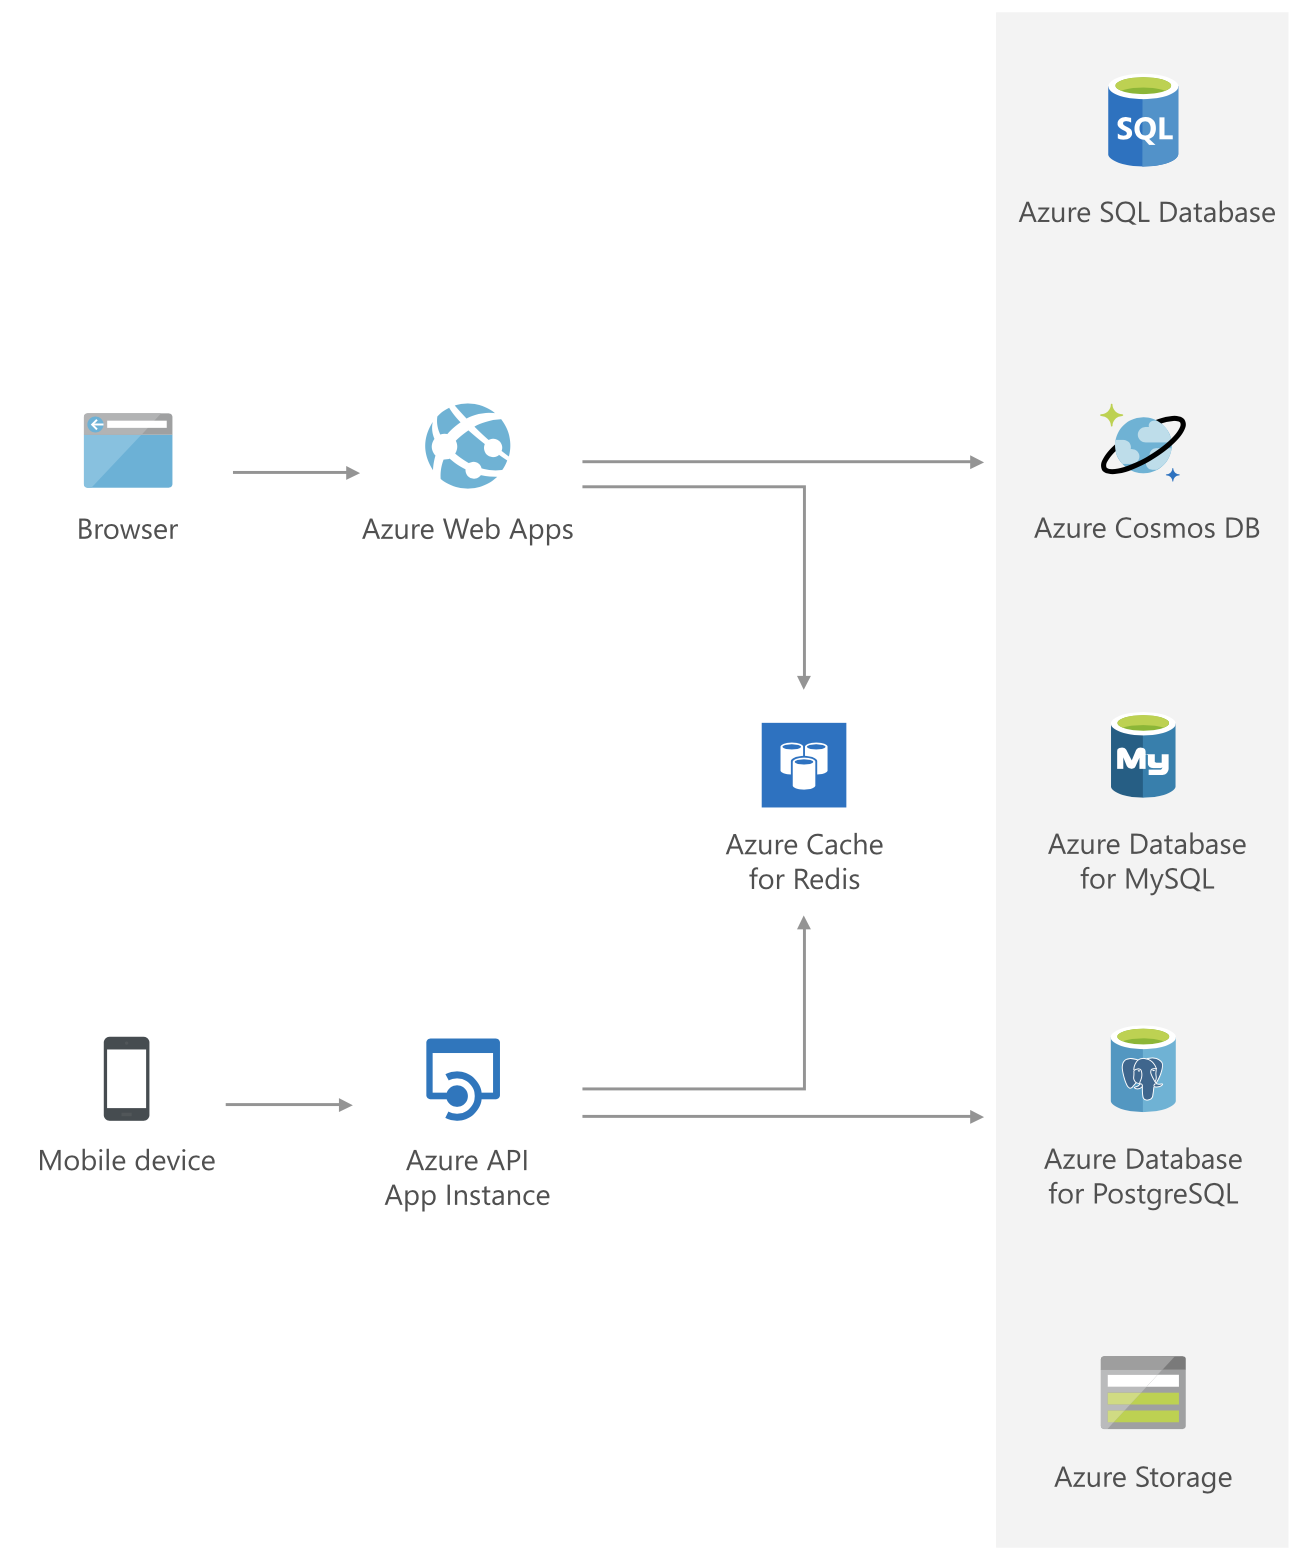
\includegraphics[width=0.5\linewidth]{cacheForRedis-integration}}%
	\caption{Azure Environment Integration}
	\label{fig:azure_ecosystem}
\end{figure}

\subsection{Aerospike}
\label{ssec:aerospike}

Aerospike \cite{aerospike:1} is an enterprise-grade, high performance Key-Value Store. It is another \gls{KVS} technology currently available today. It promises a philosophy of \textit{"no data loss" } through Strong Consistency. Normal systems trade requiring this type of consistency usually trade performance for data integrity but Aerospike allows it  with minimal performance loss. That means it can be used for example in banking payments, retail and telecommunications use cases.

It also provides a dynamic cluster management and unique flexible storage. That enables very easy deployments and particularly very easy scalability, so it is able to meet any data volume needs and still maintaining low latencies across that wide range of data volumes, from low volumes until hundreds \gls{TB} of data.

As for security, it includes (the enterprise version) a database access management and audit trail logs. It also includes transport level encryption for client-server traffic and cross-datacenter traffic \cite{aerospike:2}.

\subsection{Discussion}
\label{ssec:s1_discussion}

In this chapter when gather information about the overview of th current Key-Value Store. We can conclude that the most important feature of this technology is the performance and all of the above products mentioned do focus on that characteristic. Some of them even compromise in another features to achieve the best performance possible. Security is not the main concern and the most used measures in the current technologies being securities implementations at the network and transport level by using \gls{TLS} and also full disk encryption. 

Network and transport layer security is a must when implementing any system, and this thesis will also use those standards. 

As for full disk encryption on the server, it opens up some attack vectors. Full disk encryption means that random users will not be able to query the data but credentialed users can. Although, anyone with full access to the database, for example database operators or/and administrators, can decrypt and access all information. This creates a risk of privacy breaking due to hackers wielding stolen credentials, rogue insiders who have been granted more access than they need or the well known honest-but-curious adversary model, where an administrator with full credentials does not have bad intentions, but, driven by curiosity, access information therefore breaking data privacy. A cloud based \gls{KVS} service like the ones talked above, this type of vulnerabilities can be a major concern for a use case with very sensitive data since the server would be off premises, there is no control over it when it comes to privacy of data.

This thesis will implemented a system based on Redis, the most popular and used Key-Value Store currently used and will try to solve some of the problems with security described above. It will compare the principle feature of a \gls{KVS}, the performance, of a simple and normal Redis server and a privacy-enhanced Redis solution so the user can calculate the trade-off between performance and security and applied the correspondent solution to their own use case.

\section{Trusted  Computing Environments} % (fold)
\label{sec:trusted_computing _environments}

Modern data processing services hosted in the cloud are under constant attack from malicious system administrators, server administrators and hackers who exploit bugs on applications, operating systems or even the hypervisor. However, current days shows a massive trend of business moving to the cloud infrastructure looking for easy deployment, managed services with built-in replication and fault tolerance, fast and trivial scaling and predicted costs.

With more and more data exposed in the cloud, hackers have a bigger desire to exploit and look for vulnerabilities. This results in frequent data breaches that reduce trust in online services. The need for cloud providers to ensure a level of security and trust to make the user comfortable of moving its data to the cloud has never been bigger, and with that need some solutions in the form of Trusted Computing Environments (\gls{TCE}) appeared.

Trusted Computing is a concept that strives to provide strong confidentiality and integrity guarantees for applications running on untrusted platforms. It forces a certain machine to behave an expected way even if running on a remote or machine that is out of our control.

\gls{TCE} will also provide a decrease of the Trusted Computing Base (\gls{TCB}) - the amount of components that the application needs to trust in order to run smoothly. By isolating the service running on this trusted environments (limiting the set of instructions available and encrypting data), it prevents the operating system, the hypervisor and even malicious system administrators (three components normally on the \gls{TCB}) to break data confidentiality and integrity within this environments.

There are a few hardware/software based solutions to achieved a trusted computing environment, and they will be explained in the next sections.

\subsection{TPM – Trusted Platform Modules } % (fold)
\label{ssec:trusted_platform_modules}

A Trusted Platform Module, also known as a \gls{TPM} is a technology proposed by the Trusted Computing Group (\gls{TCG}) designed to provide hardware-based security related functions. It's a chip embedded into the motherboard and includes multiple security mechanisms to make it tamper resistant to physical harm and malicious software is unable to mess with its security features \cite{tpm:1}. Some key advantages of using \glspl{TPM} are:

\begin{itemize}
	\item Generate, store, and limit the use of cryptographic keys
	\item Platform identity by using the TPM’s unique RSA key, which is burned into itself also known as Endorsement Key (\gls{EK}) and never leaves the \gls{TPM}.
	\item Help ensure platform integrity by taking and storing security measurements.
\end{itemize}

Figure \ref{fig:tpm_architecture} shows the mains components and services provided by a \gls{TPM} module. As shown in the figure, all of them only have one access point \gls{I/O} which is protected and safely managed by the \gls{TPM} execution engine.

\begin{figure}[htbp]
	\centering
	{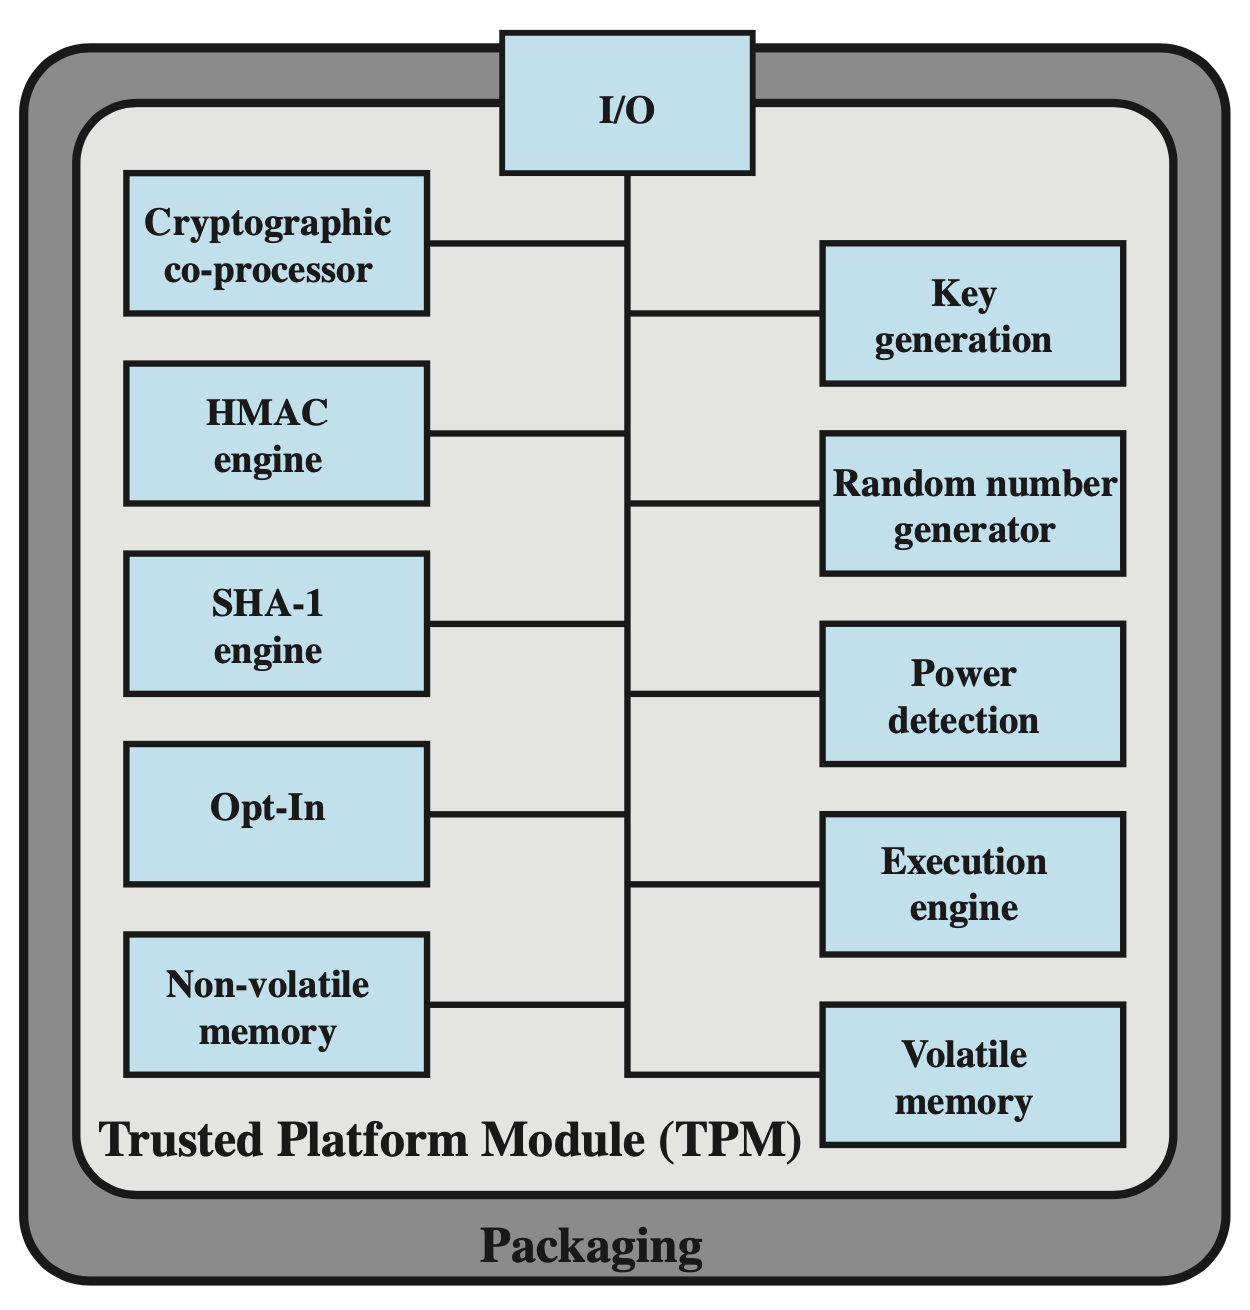
\includegraphics[width=0.5\linewidth]{tpm-architecture}}%
	\caption{TPM insides}
	\label{fig:tpm_architecture}
\end{figure}


With all the components described by figure \ref{fig:tpm_architecture}, \glspl{TPM} provide there main \gls{TPM} features: Encryption, Authenticated Boot and Attestation. 

The first feature is used for every security and confidentiality aspects, mainly generating cryptographic keys, encrypting, signing and hashing data with secure standard algorithms melted in the module.

Authenticated Boot is the ability to boot the \gls{OS} in stages, assuring that each portion of OS, as it is loaded, is a version trusted and approved for use, detecting hardware and software changes on every stage to verify if the code loaded can be trusted. This boot sequence happens with the help Platform Configuration Registers (\gls{PCR}) that store the trusted software hashes.

The attestation feature is a way for a client to remotely check the state of a machine and will be further explained in the next subsection.


\subsection{TPM - Enabled Software Attestation} % (fold)
\label{ssec:enabled_software_attestation}

The remote attestation feature of a \gls{TPM} is the ability of a program to authenticate itself against external verifiers. Is a mechanism that allows a remote party to verify the internal state of the OS or another software and decided whether or not that piece of software is intact and trustworthy. The verifier can trust that the attestation data is accurate and not tampered with because it is signed by the internal key of the \gls{TPM}, a special key known as the Attestation Identity Key, known from now on as \gls{AIK} \cite{attestation:aik}.

A remote attestation procedure is described in image \ref{fig:remote-attestation} \cite{attestation:1}: 

\begin{figure}[htbp]
	\centering
	{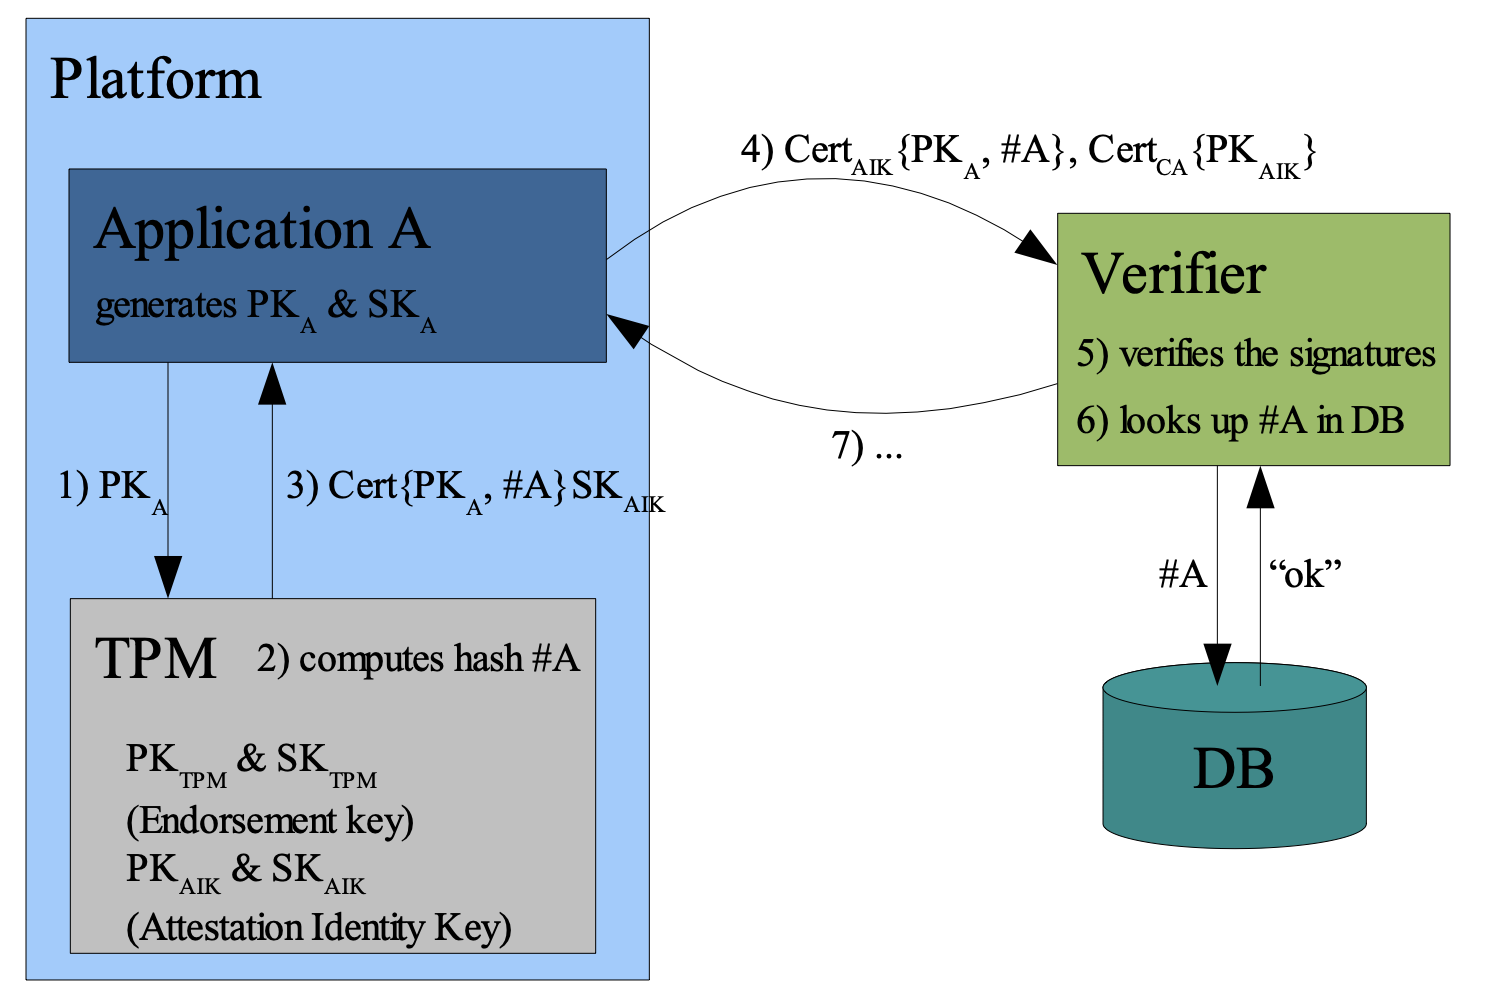
\includegraphics[width=0.5\linewidth]{remote-attestation}}%
	\caption{Remote Attestation Procedure}
	\label{fig:remote-attestation}
\end{figure}

\begin{enumerate}
	\item The application “A” generates a public/private key pair PK\textsubscript{A} \& SK\textsubscript{A} and asks the \gls{TPM} to certify it.
	\item The TPM computes a hash value \#A of the executable code of program “A”.
	\item The TPM creates a certification including PK\textsubscript{A} and \#A and signs it with the attestation identity key SK\textsubscript{AIK}.
	\item When application “A” wishes to authenticate itself to a remote party, it sends the cert. of its public key and hash value \#A along with a cert. issued to the TPM by a trusted certification authority (\gls{CA}).
	\item The remote party verifies the cert. chain.
	\item The remote party looks \#A up in a database which maps hash values to trust levels.
	\item If application “A” is deemed trustworthy, we continue the communication,
	probably by using PK\textsubscript{A} to establish a session key.
\end{enumerate}

\subsection{HSM – Hardware Security Modules} % (fold)
\label{ssec:hardware_security_modules}

An (\gls{HSM}) hardware security module is normally an external module that can be added to a system, in form of a \gls{USB} device or a component living in a secure network as a trusted server, instead of being embedded into the motherboard like a \gls{TPM}. It provides a dedicated system of hardware enable accelerated cryptographic functions like encryption, decryption, key generation and signing capabilities \cite{hsm:1}

What makes this devices so secure, like the \gls{TPM}, is it can´t be interfered with by external code, and it provides an array of protective mechanisms to detect and prevent external physical tampering like drill protection foil, resin-embedded chips as well as temperature and voltage sensors. Any detection of tampering will result in an alarm as well as countermeasures by the applications installed inside. \cite{hsm:2}.

\gls{HSM} can have various applications and can be used in simple forms for example a specific bank dongle that generates \gls{OTP} (one-time password) for accessing your account or be a big corporation and enterprise appliance in various industries, e-health, automotive and \gls{IoT} systems.

\subsection{Trusted Execution Environments} % (fold)
\label{ssec:trusted_execution_environments}

A Trusted Execution Environment (\gls{TEE}) is an abstraction that describes a machine
capable of executing a given program P in isolation, i.e. whose output is determined by
the initial state of P and a set of defined inputs given into the \gls{TEE} (Barbosa et al., 2016).

It is a secure area of the main processor that ensures sensitive data and code loaded inside is stored, processed and protected in an isolated and trusted environment. As such, it offers protection from software attacks even the ones generated in the operating system.

A \gls{TEE} guarantees that: 
\begin{itemize}
	\item The code loaded in the environment is authentic and was not tampered by an attacker.
	\item All system state is correct (CPU registers, memory and sensitive I/O).
	\item The code, all data generated and runtime state is confidential and stored persistently.
\end{itemize}

The threat model of a \gls{TEE} should include all software attacks and the physical attacks performed on the main memory and its non-volatile memory.

"There are many interpretations of what is meant by Trust. In the \gls{TEE} it is used to imply that you may have a higher level of trust in validity, isolation and access control in items (assets) stored in this space, when compared to more general purpose software environments" \cite{tee:1}.

\subsection{Intel SGX} % (fold)
\label{ssec:intel_sgx}

"Intel® Software Guard Extensions (Intel® SGX) is a set of instructions that increases the security of application code and data, giving them more protection from disclosure or modification." \cite{sgx:3}.

These set of instructions are one of the latest iterations of trusted computing solutions and designs that tries to tackle the problem of securing remote computations by leveraging secure hardware on the remote host machine. The SGX processor enables a secure container called enclave which protects the confidentiality and integrity of the execution, such as code and data while relying on software attestation mechanisms.

A \gls{SGX} can be though as a reverse sandbox. With a sandbox you are trying to protect the system from your application, but with \gls{SGX} you are trying to do the opposite and protect the application from the system. The system can be the \gls{OS}, the hypervisor, the BIOS, the firmware or even the drivers \cite{sgx:2}.

A \gls{SGX} enabled application is broken into two parts, the untrusted and trusted parts. The trusted part of the application is all the processing that deals with any sensitive data the application is handling. This part will be run inside enclaves and be stored in protected memory. The rest will live in normal memory and not be protected.

It provides this kind of security from the hardware by isolating all the private data from the outside, placing it into a restricted area of the memory called the \gls{PRM} more specifically in the \gls{EPC} (Enclave Page Cache) as shown on figure \ref{fig:sgx_memory_architecture}. The \gls{PRM} is a zone of the \gls{RAM} with guaranteed access management by the CPU where it will deny every external access and only allow access through the associated enclave. This region of the memory is also known as the private/protected memory or the trusted part of the application.

\begin{figure}[htbp]
	\centering
	{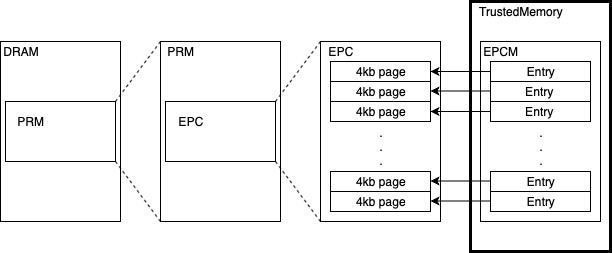
\includegraphics[width=1.0\linewidth]{sgx_memory_architecture}}%
	\caption{\gls{SGX} Memory Archicecture \cite{sgx:4}}
	\label{fig:sgx_memory_architecture}
\end{figure}

Because the \gls{SGX} enclaves execute within the virtual address space of a process, the translation of enclave addresses must be trusted. However, since it is the \gls{OS} that manages the translation between physical and virtual addresses (and the \gls{OS} cannot be trusted), \gls{SGX} maintains an internal data structure called the \gls{EPCM} (Enclave Page Cache Mapping) which tracks the referred mapping as well as the information described on figure \ref{fig:sgx_memory_architecture} \cite{sgx:5}.

With all this information about enclave pages, the processor can now performed a controlled access management to the enclave page cache described in figure \ref{fig:sgx_access_control}, where it will denied access  not only from outside the enclave but as well as from enclaves that do not own the page of memory request creating then, an isolated memory region.

\begin{figure}[htbp]
	\centering
	{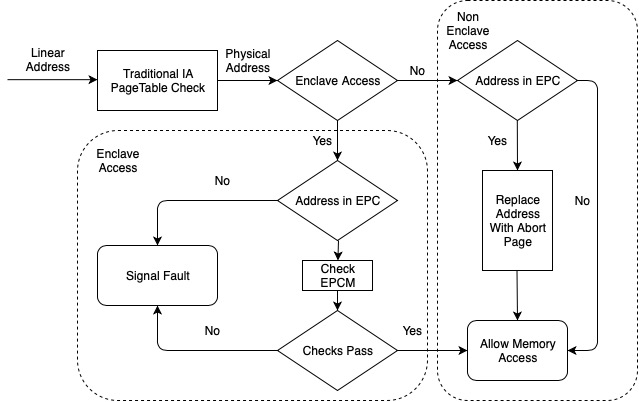
\includegraphics[width=0.8\linewidth]{sgx_access_control}}%
	\caption{\gls{SGX} Access Control \cite{sgx:4}}
	\label{fig:sgx_access_control}
\end{figure}

The \gls{SGX} will create an enclave when sensitive code needs to run by a specific \gls{SGX} CPU instruction (ECREATE) and will create a unique instance of an enclave, establishing the linear address range and load the sensitive code into an \gls{EPC} inside the protected memory. Once all pages are loaded into the EPC, and the loading in complete, an authentication hash is computed and is available for remote attestation so a user can verify that the code running in the enclave has not been tampered with.

An enclave must expose an \gls{API} for the application to call in and advertise what services provided by the untrusted domain are needed. This is the definition of an interface boundary between the untrusted part of the code and the enclave and it is how they communicate. An \gls{Ecall} is a function that the untrusted part application can call to execute some code inside the enclave and since it exposes a sensitive interface, to reduce the enclave attack surface, the number of \glspl{Ecall} should be limited. On the other hand, the \gls{Ocall} is a function that an enclave can call to reach a service/interface outside the enclave, on the untrusted \gls{OS}. Again, calling some service out of the enclave can carry additional security risks and should be as minimal as possible \cite{sgx:6}.

When running, the execution always happens in protected mode, and to prevent data leaking, the CPU will not directly address an interrupt, fault or VM exit, but will instead emit another specific instruction (EEXIT) to properly exit the enclave, save CPU state into the enclave and only then will service the fault.

With all this properties, Intel® through \gls{SGX} set of instructions and implementation tries to achieve a secure and trusted environment with guarantees of code and data isolation, confidentiality and integrity from attackers such as the \gls{OS}, hypervisor, any hardware and even physical attacks \cite{cryptoeprint:2016:086}.

\subsection{Sanctum} % (fold)
\label{ssec:sanctum}

Sanctum \cite{cryptoeprint:2015:564} is an open-source project that shares the same as goal as Intel \gls{SGX}, providing strong provable software isolation to protected the data from external hardware and software, but claims to be simpler and protect against indirect attacks called side channel attacks \cite{Khan2014} such as cache timing attacks \cite{cachetimingattaks:1} that have been know to exist in \gls{SGX} \cite{Gtzfried2017} \cite{2017arXiv170208719S}. These are additional software attacks that can infer private information by analysing a program’s memory access patterns.

Following the minimal and simple concepts, it uses minimal invasive hardware and it does not required any modifications to the CPU major blocks, but only adds hardware to the interfaces between blocks. This allows for a respectable overhead by maintaining normal clock speeds as it does not modify the CPU core critical execution path.

Sanctum project builds on the \gls{SGX} programming model and implements an architecture that deviates as little as possible from the one built by Intel. Although it differs from \gls{SGX} by implementing the enclaves via a small combination of hardware extensions to RISC-V (an open source set of CPU instructions \cite{Waterman14therisc-v}) and a trusted piece of software called the security model, as SGX implements them via hardware microcode and presents a set of CPU instructions to manage the enclaves.

This security monitor is the core of the project and configures the hardware to enforce low-level rules that controls the enclaves's access policies. As explained in the Sanctum paper, "\textit{the security monitor checks the system software’s allocation decisions for correctness and commits them into the hardware’s configuration registers}". One of the examples and the main points of upgrade compared to \gls{SGX} is that Sanctum keeps the enclave page tables inside enclaves memory, protecting the system against the timing attacks referred above by keeping the page table dirty and accessed bits private. Their hardware extensions make sure that enclaves page tables only point to enclave memory and untrusted OS tables only point to Os memory regions and never to enclave private memory.

Sanctum is also open to the public which makes easier for security researchers to audit and find vulnerabilities and to further encourage the analysis of the code, Sanctum security monitor is written in portable C++ code and can be used across different CPU implementations.

\subsection{ARM Trust Zone} % fold
\label{ssec:arm_trust_zone}

ARM Trust Zone \cite{armtrustzone:1} is a technology that offers a system wide approach to security based on hardware enforced isolation built into the CPU \cite{armtrustzone:2}. The principle of the technology is to separate the trusted and untrusted by two virtual processors backed by hardware access control. The two states are referred as worlds, where the first is called the secure world (SW) and the other is the normal world (NW) like figure \ref{fig:armtrustzone_stack} shows.

\begin{figure}[htbp]
	\centering
	{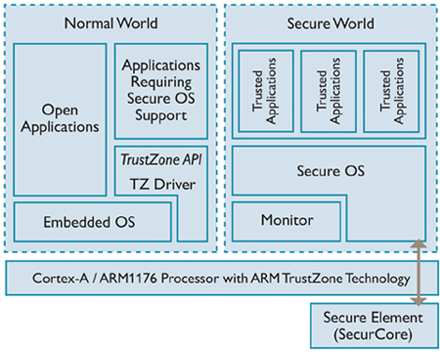
\includegraphics[width=0.5\linewidth]{ArmTrustZone_Stack}}%
	\caption{Arm TrustZone Stack \cite{armtrustzone:3}}
	\label{fig:armtrustzone_stack}
\end{figure}

The non-secure world (or normal world) is where the \gls{OS} and most of the software and applications will be running, as for the secure world is where more secure and sensitive software will run and will ensures that vital information is not intercepted by a third party. The security is enforced because each of the worlds acts isolated from the other as a runtime environment with separated resources such as memory, processor, cache, controllers, interrupts. The ARM hardware has separate copies of the registers for each worlds and cross-world register access is blocked. However the Secure Monitor shown in figure \ref{fig:armtrustzone_stack} can access non secure registers while running in secure world. This means that the monitor can then implement context switching between both worlds.

When in Normal World, the application calls a specific ARM instruction call SMC (Secure Monitor Call) to call back inside the secure world and execute in code in a secure manner.

By keeping the worlds separated from each other, the ARM TrustZone can keep applications running in secure mode isolated from the normal world applications such as the OS and thus achieving another implementation of a \gls{TEE}.

\subsection{Discussion}
\label{ssec:s2_discussion}

The \gls{TCB} (Trusted Computing Base) is the of set computer components (hardware), software and data that we need to trust and deem as not malicious in order to use a system. It's a group of various elements that are critical to a systems security in a way that any bug or vulnerability occurring from inside the \gls{TCB} components might compromise the security and privacy of the entire system. On the other hand, security flaws and bugs from outside of the ~\gls{TCB} should not become a security issue.

Hardware security like \glspl{TPM} and \gls{TEE} technologies have the goal to drastically reduce the \gls{TCB} of a system, for example, remove the \gls{OS} from the trusted base to make sure that a remote compromised machine vulnerability does not affect the security and privacy of a application or system.

By isolating the program from outside and uncontrollable sources like cloud infrastructures \glspl{OS}, hypervisors and hardware we can more safely deploy sensitive applications to those cloud providers.
That is the goal of all different implementations of trusted execution environments like the Intel \gls{SGX} and the ARM TrustZone.

Although not free of some problems, \gls{SGX} implementation of a \gls{TEE} seems to be the most accepted technology, with serious and skilled developers and security researches always working to mitigate any vulnerability in order to create a truly trusted and isolated environment.

\section{TEE/SGX Enabled Key Value Stores} % (fold)
\label{sec:sgx_enabled_key_value_stores}

There has been an increase trend from developers to move their applications to the cloud. It provides dynamically and almost seamlessly scaling with predict cost. Although it also means that users need to rely on the cloud providers for securing and maintaining the integrity of their applications. That means the user must trust not only the provider's staff but also its globally distributed software and hardware not to expose their private data. Today's cloud providers only aim to protect their privileged code from the untrusted code (the user's code) and do not provide any guarantees about the opposite scenario.

To mitigate this use case, and after studying and discussing the Key-Value stores technologies and also the trusted platform modules as well as the trusted execution environments, in this chapter, it will be presented how are this two topics being combined and used together. 

It will be more focused on the Intel SGX platform as it is the one that will be used throughout this thesis. Currently, there are a number of databases who leverage this technology to provide a more secure environment and service. In the this chapter it's presented how they work and operate, discussed the differences between them and also the how the work planned to be performed on this thesis will solve some of the problems and caveats. 

\subsection{Trusted Execution with Intel SGX}
\label{ssec:trusted_execution_with_sgx}

As explained before, Intel SGX provides a trusted execution environment by running code inside the enclaves. It creates an isolated environment where we can run some instructions as securely as possible, without \gls{OS} intervention.

Key-Value Stores and other database type systems can leverage this secure and isolated environment to perform queries on very sensitive data that would otherwise be vulnerable to some attacks. There are a few techniques currently implemented to use isolated environments. Maintaining an encrypted database and using enclaves cryptographic capabilities to decrypt data and perform queries on plain text with the assurance of no data leaking is a possible use case. Also, maintaining a database fully on enclave memory, where it cannot be access by anyone other than the CPU is another way to keep the data secure by leveraging isolated and trusted execution environments. Different techniques will be furthermore discussed bellow. 

As we can see, isolated and trusted execution environments are an important feature when it comes to protecting the data from the \gls{OS} and Key-Values Store systems do benefit from them.

\subsection{Circumvention of SGX Limitations}
\label{ssec:circumvention_of_sgx_limitations}

There are a few limitations and challenges of the SGX platform that we address when programming for such technology.

It starts with a big challenge of choosing and defining what parts of the program can benefit of the \gls{SGX} security. As it is known, it works with two major application components, the trusted and untrusted modules of or program. The limitations have to be thoroughly analysed so we can make that definition.  

The main limitations are: 

\begin{itemize}
	\item Performance
	\item Memory
	\item \gls{I/O}
	\item \glspl{syscall}
\end{itemize}

In the \gls{KVS} world, as we extensively covered, performance is the major concern and there is no real way around this limitation. Using secure enclaves will definitely decrease the supposed blazing fast performance. Although, with intelligent partition between the untrusted code, which will be fast, and the trusted instructions, which will be slower we can limit the performance overhead. By separating and well defining both modules of the application, we can decrease the code that needs to run securely and find a fine compromised between security and performance.

Memory sizing is also a limitation when using enclaves in \gls{SGX} technology. The amount of private secure data that can be maintained by the enclave is limited to the size of the enclave cache, which is around 128 \gls{MB}, being that only about 94 \gls{MB} are available to the application, with the rest reserved to metadata. Now, with \gls{SGX} v2 and for some operation systems, mainly Linux because of paging swap support, it can be increased up to all the memory available in the system \cite{sgx:1} by swapping pages from the \gls{EPC} to main untrusted memory, with guaranteed of confidentiality, integrity and data freshness. When evicting pages from the \gls{EPC}, it is assigned a unique version number which is recorded in a new type of EPC page and the contents of the page, metadata, and EPCM information are encrypted and written out to system memory. When reloading a page back into \gls{EPC} the page is decrypted and has its version and integrity checked to make sure it was not tampered with.

Although, page eviction to main untrusted memory introduces a big overhead because of encryption and decryption and integrity checks (2x - 2000x) \cite{scone:1}. Clever partitioning of the application into the untrusted and trusted modules will help to overcome this limitation as described in the next sections.

\gls{I/O} and \glspl{syscall} are limited by default on the enclave for security purposes, so it can't affect or be affected by the \gls{OS}. There is a way to perform and access \gls{I/O} and \glspl{syscall} through the aforementioned \glspl{Ecall} and \glspl{Ocall} (section \ref{ssec:intel_sgx} of this thesis), but they have to be accounted for when implementing the application.

\subsection{SGX-Enabled Secure Databases}
\label{ssec:sgx_enabled_secure_databases}

Database management service developers are now implementing secure databases ready to take advantage of Intel \gls{SGX} hardware. It differs from normal databases because it runs on top of protected and encrypted memory so it can work with minimal \gls{TCB}.

Next subsections present and discuss the overview of the current technology that leverages \gls{SGX} to provide a secure database.

\subsubsection{EnclaveDB}
\label{sssec:enclave_db}

EnclaveDB \cite{enclavedb:1} is a privacy enhanced and secure database that works alongside with Intel \gls{SGX} and provides a Structured Query Language (SQL). It uses its technology to maintain all sensitive information inside \gls{SGX} enclaves in order to keep them secure from a threat model of strong adversaries that can control the entire software stack  on the database server. It resists attack from the administrator server, the database administrator and attacker who may compromised the operating system, the hypervisor or the database server.

Following Intel's application guidelines, EnclaveDB has a two part architecture: trusted (running on the enclave) and untrusted modules. The enclave hosts a query processing engine, natively compiled stored procedures and a trusted kernel which provides API's for sealing and remote attestation. The untrusted host process runs all other components of the database server. Figure \ref{fig:enclaveDB_architecture} shows the architecture of the enclaveDB server-side.

\begin{figure}[htbp]
	\centering
	{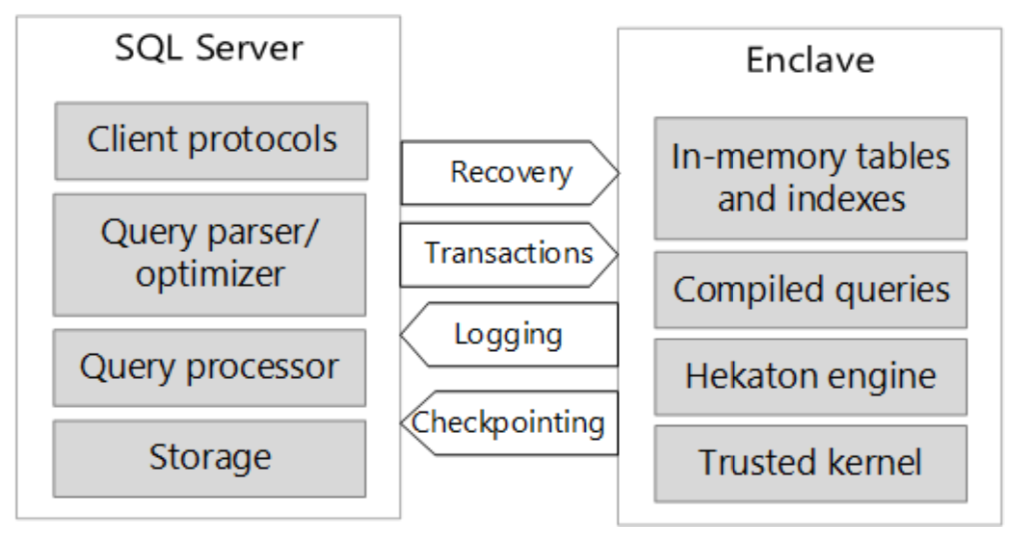
\includegraphics[width=0.5\linewidth]{enclaveDB_architecture}}%
	\caption{Server-side components of EnclaveDB}
	\label{fig:enclaveDB_architecture}
\end{figure}

Leveraging \gls{TEE}, EnclaveDB then provides a database with a \gls{SQL} interface and guarantees confidentiality and integrity with low overhead. With its design it also reduces the \gls{TCB} to a smaller set than any other "normal" database.

\subsubsection{Pesos DB}
\label{sssec:pesos_db}

Pesos \cite{pesos:1} is a secure implementation of object storage services like Amazon S3 \cite{s3:1}, Azure Blob Storage \cite{azureStorage:1}, Google Cloud Storage \cite{googleStorage:1} among others. In these current large-scale services, due to their complexity, the risk of confidentiality and integrity violations increase significantly. This storage systems are characterised by multiple layers of software and hardware stacked together which means the access policies for ensuring confidentiality and integrity are scattered across different code paths and configurations, thus exposing the data to more security vulnerabilities. Furthermore, untrusted third-party cloud platforms expose an additional risk of unauthorised data access by a malicious administrator.

Pesos allows clients to specify per-object security policies concisely and separately from the remaining storage stack. It also provides cryptographic attestation for the stored objects and their associated policies to verify the policy enforcement.

It enforces this policies by leveraging the Intel \gls{SGX} for trusted execution environments and Kinetic Object Storage \cite{kinetic:1} for trusted storage (secure storage - not the focus of this thesis). It structures a policy-compiler, its binary-format interpreter, per-object policy metadata, and the enforcement logic into a single layer of the storage stack. With this unification, it drastically reduces the \gls{TCB} when compared to the order cloud services. Then it uses the trusted execution environment provided by \gls{SGX} to connect directly Kinetic disk through an encrypted Ethernet connection allowing for object transfer and policy enforcement securely without any intermediate layers in the storage stack.

\subsubsection{Speicher}
\label{sssec:speicher}

Speicher \cite{speicher:1} is a secure \gls{LSM}-based Key-Value store that uses Intel \gls{SGX} and it ensures not only strong confidentiality and integrity properties, but also data freshness to protect against rollback/forking attacks. It leverages \gls{SGX} technology to achieve those security characteristics focusing on providing a \textbf{persistent} service, tolerant to system faults and securely recovering from crashes. It also tackles in interesting ways, two of the major limitations of \gls{SGX}: Memory Limits and Performance.

Implementing a Key-Value Store has a major requirement - High performance and low latency queries for big data structures. As already discussed, \gls{SGX} has some memory limits. The enclave memory is located in the Enclave Page Cache (\gls{EPC}) which is limited to 128 \gls{MB} with about 94 \gls{MB} available for application use (the rest being reserved for metadata). To allow creation of enclaves with bigger size than \gls{EPC}, the \gls{OS}  can use secure paging mechanism where it evicts pages to untrusted memory. Although with page encryption, decryption and integrity checks, this solution introduces high overheads (2× - 2000×) \cite{scone:1}.

To address this performance and memory problems, the developers of Speicher implemented the following custom features (from Speicher public paper):

\begin{itemize}
	\item \textit{"\textbf{I/O library for shielded execution}: Direct \gls{I/O} library for shielded execution. The \gls{I/O} library performs the \gls{I/O} operations without exiting the secure enclave; thus it avoids expensive system calls on the data path."}
	
	\item \textit{"\textbf{Asynchronous trusted monotonic counter}: Trusted counters to ensure data freshness. The counters leverage the lag in the sync operations in modern \gls{KVS} to asynchronously update the counters. Thus, they overcome the limitations of the native \gls{SGX} counters."}
	
	\item \textit{"\textbf{Secure \gls{LSM} data structure}: Secure \gls{LSM} data structure that resides outside of the enclave memory while ensuring the integrity, confidentiality and freshness of the data. Thus, the \gls{LSM} data structure overcomes the memory and \gls{I/O} limitations of Intel \gls{SGX}."}
\end{itemize}

The technology leverages \gls{SGX} with a clever partition between trusted and untrusted modules of the application. By maintaining the encrypted data on untrusted memory hardware it addresses the memory and persistent limitations, and by keeping some information in secure enclave memory and with a good \gls{I/O} library it overcomes (to an extent) the performance issues.

\subsubsection{ShieldStore}
\label{sssec:shieldstore}

ShieldStore \cite{shieldstore:1} is a \textit{"(...) shielded in-memory Key-Value Storage with \gls{SGX}"}. It aims to provide a very fast and low latency queries over very large data trying to overcome the \gls{SGX} memory limitation. It accomplice's it by maintaining the majority of the data structures in the non-enclave memory region, addressing as well the performance issue by not relaying on the page-oriented enclave memory extension provided by \gls{SGX}.

ShieldStore runs server-side in the enclave to protect encryption keys and for remote attestation and it is used to perform all the \gls{KVS} logic. It uses a hashed index structured but places it in the unprotected memory region instead of the enclave \gls{EPC}. As the main data structure is not protected by the \gls{SGX} hardware, each data entry must be encrypted by ShieldStore in the enclave, and written to the main hash table.

The main flow and architecture is as described on figure \ref{fig:shieldstore_overview}.

\begin{figure}[htbp]
	\centering
	{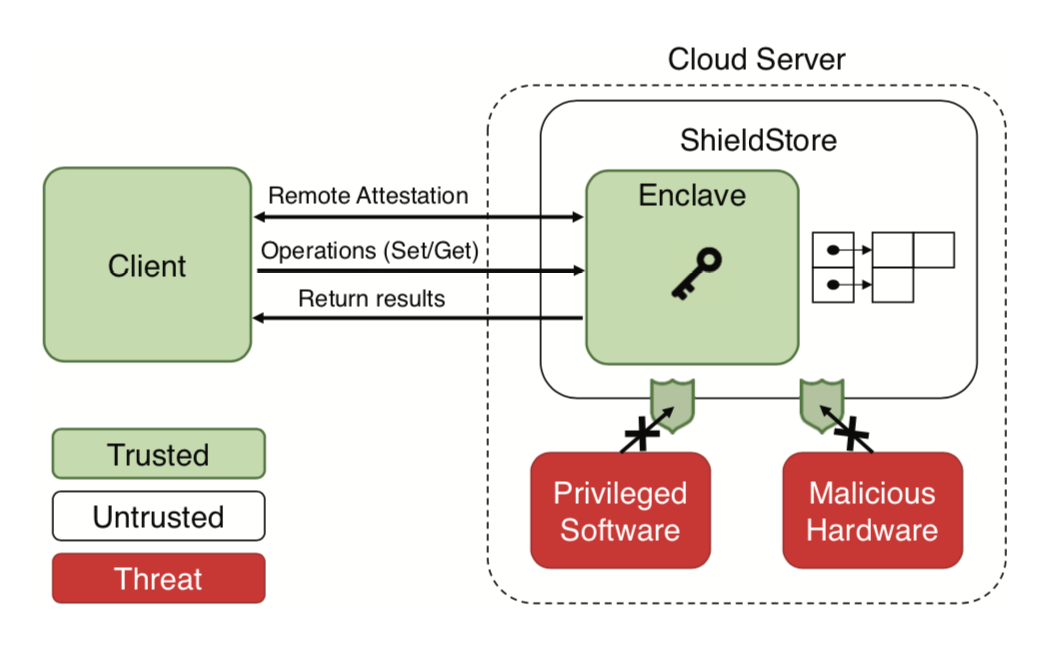
\includegraphics[width=0.5\linewidth]{shieldstore_flow}}%
	\caption{Overview of ShieldStore}
	\label{fig:shieldstore_overview}
\end{figure}

First the client remote attests the server-side (1) verifying \gls{SGX} support of the processor, the code, and other critical memory state of an enclave. In a second step, the client and the server exchange sessions keys (2) in order to establish a secure connection, using Intel \gls{SGX} libraries to do so. Using this newly generated session key, the client sends a request for an operation (3). The server deciphers and verifies the request and accesses the Key-Value Store (4). Clients do not access the server-side ciphertexts neither need to know the encryption key used by the server to encrypt the values. The server will then decrypt the data from the storage, encrypted it again with the session key and reply to the client (5). All accesses to the \gls{KVS} have integrity checks.

\subsection{Discussion}
\label{ssec:s3_discussion}

Concluding, EnclaveDB (section \ref{sssec:enclave_db}) and Pesos (section \ref{sssec:pesos_db}) presents secure databases and objects storage systems respectively, using \gls{SGX}, but EnclaveDB assumes that \gls{SGX} supports large enclaves whose size is an order of several hundred \glspl{GB} and Pesos restricts the size of data structure to the size of \gls{EPC}. On the other hand, Speicher (section \ref{sssec:speicher}) and ShieldStore (section \ref{sssec:shieldstore}) proposes a store that alleviates the memory limitation of Intel \gls{SGX} by storing encrypted data on untrusted memory regions. Speicher and ShieldStore have similar architectures, but the former is primarily design for persistence storage and the latter is focused on a fast in-memory key-value store.

We can now conclude that the clever partitioning of the application into trusted and untrusted parts is really important when programming with Intel \gls{SGX}. It directly affects \glspl{syscall} and \gls{I/O}, performance and memory of the service. 

The long goal of this thesis is to implement a system with characteristics from the databases present above. In terms of performance we plan to implement partial homomorphic encryption, so it allows to perform operations directly over in-memory encrypted data. This will be a challenge, as fully homomorphic encryption is not yet practical \cite{homomorphic:1}, so adaptations must be made, but performance increase are expected  over the databases presented above, by not needing to decrypt the data in secure execution. Persistence will also be a requirement just like some of the databases presented.

For trusted execution with \gls{SGX}, extensive research is needed to partition the application in the two necessary modes to circumvent persistence, performance and memory \gls{SGX} limitations. It will also be researched and tested the ability to provide built-in replication and availability with \gls{SGX}.

\section{Related Work Balance and Critical Analysis}
\label{sec:related_work_balance_and_critical_analysis}

In the current days, computer scientists are always looking for a secure, fast and cheap environment to develop applications. As we know, it is not feasible to have all three of this elements working flawlessly without any compromises. Although, by combining in-memory key value stores, trusted remote execution environments and cloud providers, developers can now have a practical example of what would be to develop for a privacy enhanced secure system with reduce costs by using cloud providers and with better reassurances that the hardware and software that it's out of the control of the user will have a minimal impact on sensitive data and code of an application. By adding the performance benefits of an in-memory key value store and all of its technology, like built-in security, built-in replication and persistence we can in the best of our abilities today, combine the best of the three worlds without compromising too much on any of them.

In this thesis we will compare different kinds of approaches to implement a fast system with the assurance of a secure data flow that can easily be deployed into the cloud without fear of any components out of our control.